\begin{quote}
The aim of the \emph{Peeragogy Handbook} is to establish effective
peer-learning techniques that you can implement ``on the ground.'' We
suggest that you look through the Handbook, try a few of these
suggestions, and see how they work for you. Then we invite you share
your experiences, ask for feedback, and work with us to improve the
Handbook and the field we affectionately call ``Peeragogy.''

In this part of the \emph{Peeragogy Handbook}, we ``peeragogues'' have
summarised the most important and applicable research and insights from
two years of inquiry and discussion. Although there's been no shortage
of experimentation and formal research into collaborative, connective,
and shared learning systems in the past, there is a new rumbling among
education thinkers that suggests that when combined with new platforms
and technologies, peer-learning strategies as described here could have
a huge impact on the way educational institutions evolve in the future.
We've also seen for ourselves how peer-learning techniques can help
anyone who's interested to become a more effective informal educator.
\end{quote}

%% \begin{figure}[htbp]
%% \centering
%% 
\includegraphics[width=.4\textwidth]{../pictures/peeragogy-in-action.jpg}
%% \end{figure}

\subsection{The interplay of individual and group}

``Personal'' supports ``peer''. We can consciously cultivate living,
growing, responsive webs of information, support, and inspiration that
help us be more effective learners. This is known as a personal learning
network. We'll offer tips on how to build these networks --- and we'll
also explain how strong personal learning networks can contribute to and
evolve into even stronger peer learning networks.

``Peer'' supports ``personal''. As we work together to develop shared
plans for our collective efforts in group projects, we usually can find
places where we have something to learn. Furthermore, if we are willing
to ask for help and offer our help to others, everybody's learning
escalates. Being mindful of effective interpersonal learning patterns is
an important part of building an effective personal learning plan.

\subsection{Peer learning through the ages}

As you will have guessed, our new term, peeragogy, is a riff on the word
pedagogy --- the art, science, or profession of teaching. Pedagogy has a
somewhat problematic origin: it comes from the ancient Greek tradition
of having a child (paidos) be supervised (agogos) by a slave. Greek
philosophers seem to have disagreed about to the best way for
individuals to gain knowledge (and even more so, wisdom). Socrates, who
insisted that he was not wise, also insisted that his interlocutors join
him in investigating truth claims, as peers. And yet, Plato, the most
famous of these interlocutors and the best-known author of Socratic
dialogs, in his most famous allegory of the cave, has Socrates say, with
a modest but clearly pedagogical bent:

\begin{quote}
\textbf{Socrates}: This entire allegory, I said, you may now append,
dear Glaucon, to the previous argument; the prison-house is the world of
sight, the light of the fire is the sun, and you will not misapprehend
me if you interpret the journey upwards to be the ascent of the soul
into the intellectual world according to my poor belief, which, at your
desire, I have expressed---whether rightly or wrongly God knows. But,
whether true or false, my opinion is that in the world of knowledge the
idea of good appears last of all, and is seen only with an effort; and,
when seen, is also inferred to be the universal author of all things
beautiful and right, parent of light and of the lord of light in this
visible world, and the immediate source of reason and truth in the
intellectual; and that this is the power upon which he who would act
rationally either in public or private life must have his eye fixed.
\end{quote}
In more recent centuries, various education theorists and reformers have
challenged the effectiveness of what had become the traditional
teacher-led model. Most famous of the early education reformers in the
United States was John Dewey, who advocated new experiential learning
techniques. In his 1916 book, \emph{Democracy and Education} {[}1{]},
Dewey wrote, ``Education is not an affair of `telling' and being told,
but an active and constructive process.'' Soviet psychologist Lev
Vygotsky, who developed the concept of the Zone of Proximal Development,
was another proponent of ``constructivist'' learning. His book,
\emph{Thought and Language} {[}2{]} also gives evidence to support
collaborative, socially meaningful, problem-solving activities as
opposed to isolated exercises.

Within the last few decades, things have begun to change very rapidly.
In ``Connectivism: A Learning Theory for the Digital Age,'' George
Siemens argues that technology has changed the way we learn, explaining
how it tends to complicate or expose the limitations of the learning
theories of the past {[}3{]}. The crucial point of connectivism is that
the connections that make it possible for us to learn in the future are
more relevant than the knowledge we hold individually in the present.
Technology can, to some degree and in certain contexts, replace ``know
how'' with ``know where to look.''

If you want more details on the history, theories, and recent
experiments related to peer learning, we have a more extensive
literature review available. We've also adapted it into a Wikipedia
page, which you can edit as well as read.

\begin{figure}
\begin{center}
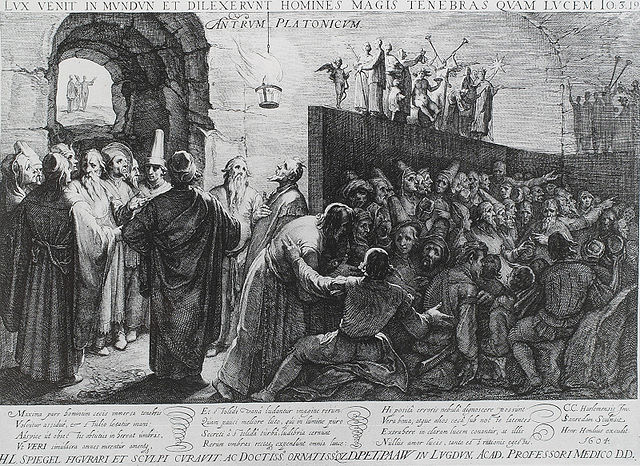
\includegraphics[width=.8\textwidth]{../pictures/plato_cave.jpg}
\end{center}
\caption*{\href{http://commons.wikimedia.org/w/index.php?title=File:Platon\_Cave\_Sanraedam\_1604.jpg\&oldid=68567627}{Platon Cave Sanraedam (1604)}. By Jan Saenredam {[}Public domain{]}, via
Wikimedia Commons}
\end{figure}

\subsection{From peer learning to peeragogy}

The idea that we needed a new theory (which we initially gave the name
``paragogy'' {[}4{]}) arose out of the challenges we faced doing peer
learning. Our aim was to understand how groups and organizations can
become better at serving participants' interests, while participants
also learn and become better contributors.

Paragogy began as a set of proposed principles that describe peer
produced peer learning -- we'll say what these principles are just
below. We designed them to contrast with a set guidelines for adult
educators advanced by Malcolm Knowles {[}5{]}. The paragogy principles
focus on the way in which co-learners shape their learning context
together. Very likely, there will be no educator anywhere in sight. And
just for this reason, peer produced peer learning is something for
``innovative educators'' everywhere. You don't need to have the word
teacher, trainer, or educator in your job title. It's enough to ask good
questions.

The paragogy principles aim to make that more explicit. They advocate
for an approach to peer learning in which:

\begin{enumerate}
\item
  Changing context is a decentered center.
\item
  Meta-learning is a font of knowledge.
\item
  Peers provide feedback that wouldn't be there otherwise.
\item
  Learning is distributed and nonlinear.
\item
  You realize the dream if you can, then wake up!
\end{enumerate}
If some of these principles seem a bit ephemeral, it may help to think
of in a more unified manner, as a set of dimensions that describe
possible changes that can take place in peer produced peer learning
{[}6{]}:

\begin{enumerate}
\item
  Changing the nature of the space
\item
  Changing what I know about myself
\item
  Changing my perspective
\item
  Changing content or connectivity
\item
  Changing objectives
\end{enumerate}
Now that we've connecting the idea of paragogy to a perspective focused
on the kinds of change that can take place in peer produced peer
learning, it's time to reveal that our secret for success is hidden in
plain view: the word ``paragogy'' means ``production'' in Greek. We're
particularly interested in how the powerful blend of peer learning and
collaborative work drives open source software development, and helps to
build resources like Wikipedia. But in fact it works equally well in
offline settings, from official hacker/maker spaces to garages and
treehouses. Projects like
\href{http://storycorps.org/about/}{StoryCorps} show how contemporary
media can add a powerful new layer to ancient strategies for teaching,
learning, and sharing.

The word ``peeragogy'' attempts to make these ideas immediately
understandable to everyone, including non-geeks. Peeragogy is about
peers learning together, and teaching each other. In the end, the two
words are actually synonyms. If you want to go into theory-building
mode, you can spell it ``paragogy''. If you want to be a bit more down
to earth, stick with ``peeragogy.''

\subsection{References}

\begin{enumerate}
\item
  Dewey, J. (2004). Democracy and education. Dover Publications.
\item
  Vygotsky, L. S. (1986). Thought and language. MIT press.
\item
  Siemens, G. (2005). Connectivism: A learning theory for the digital
  age. International Journal of Instructional Technology and Distance
  Learning, 2(1), 3-10.
\item
  Corneli, J. and Danoff, C. J. (2011), Paragogy: Synergizing individual
  and organizational learning. (Published on Wikiversity.)
\item
  Knowles, M. S. (1980). The modern practice of adult education: From
  pedagogy to andragogy. Chicago: Follett.
\item
  Corneli, J. and Mikroyannidis, A. (2011). Personalised Peer-Supported
  Learning: The Peer-to-Peer Learning Environment (P2PLE). \emph{Digital
  Education Review} 20, 14-23.
\end{enumerate}
